\chapter{UNIBO - 博洛尼亚大学}    

\section{大学简介}
Alma Mater Studiorum - Università di Bologna,博洛尼亚大学,创立于公元1088年神圣罗马帝国时期,是世界上广泛公认的、拥有完整大学体系并发展的第一所大学,被誉为“世界大学之母”。在以拉丁语为主要学术与研究通用语言的中世纪及近代欧洲,博洛尼亚大学始终保持着欧洲文化与学术发展的中心位置,并引领了欧洲大学体系的改革。官方拉丁文校名直译为“大学之母”(Alma Mater Studiorum)。1988年在430所欧洲大学校长共同签署的“欧洲大学宪章”中,博洛尼亚大学被正式宣称为欧洲所有大学的母校。

在大学900多年的历史里,涌现了众多杰出校友,包括文艺复兴时代的开拓人物但丁、提出太阳中心说的天文学家哥白尼,以及彼特拉克、丢勒、伊拉斯谟、哥尔多尼、马可尼、安伯托·艾柯、罗马诺·普罗迪、皮埃尔·保罗·帕索里尼等著名人物都曾在这里学习或执教。
 
博洛尼亚大学是全球大学高研院联盟(UBIAS)、欧洲研究型大学联盟(LERU)、同一个欧洲大学联盟(Una Europa)、国际公立大学论坛(IFPU)、科英布拉集团(Coimbra Group)、欧洲大学联盟(Europaeum)、乌得勒支网络(Utrecht Network)、中国-欧盟IRES-8合作等著名高校组织的核心成员。

博洛尼亚大学位列2023U.S.News世界大学排名第122位,2023泰晤士高等教育世界大学影响力排名第23位,2024QS毕业生就业竞争力排名第97位。

作为经历了近千年历史演变的教育机构,博洛尼亚大学的校园建筑保留了不同时期,特别是文艺复兴时期的众多特点。博洛尼亚大学曾被福布斯杂志评为全球最美的15所校园之一,2014年被世界最大的英文旅游信息出版商福多尔公司评为全球15所最值得访问的大学之一。博洛尼亚大学校园建筑面积117万平方米,总面积674万平方米,除了位于博洛尼亚的主校区之外,大学还有四个分校区,分别位于切塞纳、弗利、拉文纳和里米尼,另外在布宜诺斯艾利斯设有海外校区,在布鲁塞尔、纽约和上海设有办事处。

\section{招生公告}        

大学各学院在年末会公布来年招生公告(Bando di Ammissione),公告会详细说明来年的招生计划、招生名额、注册及考试流程,对入学流程有任何困扰的同学,请仔细查阅该公告。\\
公告的下载途径为:访问您感兴趣的专业官网,点击“Iscriversi”、随后选择“Iscriversi al Corso: requisiti, tempi e modalità”、下载“Bando di Ammissione A.A. 202X/202X”

\subsection{Studenti online网站注册}
新生必须使用自己的税号(尚未拥有税号的可使用自己的个人身份信息)在大学内部系统Studenti online上注册,得到自己的用户名及密码。随后登录,并通过此系统注册入学、报名考试、打印各类证明及查看自己大学生涯等等。请注意各专业申请的截止日期。如果考试顺利,但是错过了申请截止日期,依然会被取消入学资格。\\
网站为https://studenti.unibo.it/sol/welcome.htm,你可以扫描下方二维码访问\\
\\
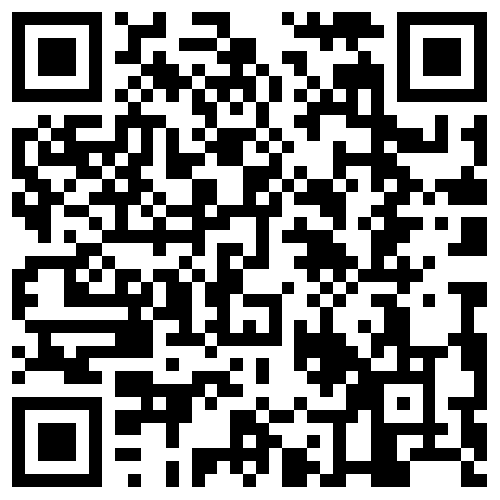
\includegraphics[scale=0.3]{studentionlineqrcode}\\
%% https://studenti.unibo.it/sol/welcome.htm

\subsection{马可波罗计划}
为中国学生提供的马可波罗计划,旨在欢迎并帮助中国学生入读意大利的大学。得益于本计划,对于想来意大利就读大学的中国学生,即使不懂意大利语也能获得入境签证。该计划要求学生在入读大学课程之前,在参与并遵守该计划的语言学校内学习10-11个月的意大利语课程。


您可以在佩鲁贾外国人大学、锡耶纳外国人大学、罗马第三大学、“Dante Alighieri”协会(即但丁语言学校)、雷焦卡拉布里亚外国人大学参加针对马可波罗计划生的意大利语课程。您还可以参加其他参与并遵守马可波罗计划的意大利大学的意大利语课程,部分私立语言学校也可以提供该课程。


\textbf{值得注意的是,}从2022/23学年起,马可波罗计划生将不再享有以往的专用名额,您需要与居住在其他非欧盟地区的学生平等竞争。\\

\subsubsection{计划生注意事项}
\begin{itemize}
\item 抵意后,必须在您预注册文件中指定的时间参加意大利语课程,不得参加非您预注册语言学校的意大利语课程。博洛尼亚大学不为马可波罗计划生提供语言培训课程 
\item 马可波罗计划生必须通过上述意大利语课程的考试,以至少达到由欧洲委员会承认的B1水平,并且获得以下意大利语证书之一:CELI B1(由佩鲁贾外国人大学颁发)、CILS B1(由锡耶纳外国人大学颁发)、PLIDA B1(由但丁语言学校颁发)和CERT.IT B1(由罗马第三大学颁发)。无论您选择的语言学校的课程进度安排如何,您都必须在2023年12月28日之前通过至少为B1水平的语言考试。
\item 如果语言学校拥有独立语言证书,则只能提供该校的语言证书。例如您在佩鲁贾外国人大学参加语言课程,则您只能提供由其颁发的CELI B1语言证书。如果语言学校没有独立语言证书,您可以提供以上四种中任意一个博洛尼亚大学认可的证书 
\item 您必须通过Studenti Online验证您的语言证书。访问Studenti Online,选择“Bandi”,随后选择“Programma Marco Polo per studenti cinesi a.a. 2023/24 - verifica certificati di lingua italiana”,上传您的语言证书和您的护照的PDF电子版。国际生办公室将对其进行审查,并在Studenti Online上发布结果。审查日期为2023年6月1日至2023年12月28日。如果因必要原因,您无法在此期间提供证书,请联系国际生办公室(internationaldesk@unibo.it)
\item 您需要在入学时,或无论如何都必须在2024年2月29日之前,将证书交付给您所就读专业的秘书处
\item 马可波罗计划生无需、也不得参加为非欧盟学生提供的CISIA意大利语测试
\item 您不能提交非上述所列的意大利语水平证明
\item 请记住,马可波罗计划生只能注册以意大利语授课的学习课程。
\end{itemize}


\subsection{入学要求}
所有专业分为:有名额限制(Numero programmato)和无名额限制(Libero accesso)两类。\\
\\
\textbf{有名额限制:}指该专业有录取名额限制,需要通过考试参与排名,按成绩高低进入录取名单(Graduatorie)后才能注册大学(Immatricolazione)。如过您的入学考试总分数或部分分数低于招生公告规定的分数线,则第一学年需要修OFA课程,在未完成OFA课程及考试前则无法进行第二学年课程的考试。\\
该类型的录取针对国际学生(居住在非欧盟地区)会有专用名额,详细信息请查看各专业的招生公告。\\
\\
\textbf{无名额限制:}指该专业无录取名额限制,无需参与排名,但招生公告中要求的考试必须参加。如果报名人数未超过意大利教育部规定的名额(取决于国际生人数名额和报名情况),则可以直接入学。如果入学考试总分数或部分分数低于招生公告规定的分数线,则第一学年需要修OFA课程,在未完成OFA课程及考试前则无法进行第二学年课程的考试。
\\
注意:部分专业的部分情况或许会有补录机会(Recupero),详情请看各专业的招生公告,补录需要自己申请!

\subsection{入学考试}

\subsubsection{本科和本硕连读(Laurea e LM a Ciclo Unico)}
分为:\\
1、需要参加TOLC考试的专业。\\
本科或本硕连读的专业都有可能要考TOLC考试,具体请通过查看自己专业的入学页面和招生公告来确定自己需要考的TOLC考试的类别。TOLC考试需要通过注册CISIA官网https://www.cisiaonline.it/,随后报名并参加考试。在通过考试后,需要参照专业的招生公告的要求参加排名(Selezione)。注意:中国学生只能参加给非欧盟学生(Studenti non UE residenti all'estero)的排名(一般为最后一次)。\\
\\
2、需要参加意大利教育部颁布的国家统一考试的专业。例如:Medicina Chirurgia、Medicina Veterinaria、Professioni di Architteto、Professioni Sanitarie etc等,阅读专业的招生公告,按步骤注册考试,在规定的日期参加考试。\\
\\
3、部分少量专业,其入学考试既不是TOLC考试也不是国家统一考试,其考试类型和方式请细读该专业的招生公告,按照其流程进行考试和入学。

\subsubsection{硕士(Laurea Magistrale)}
入学申请一般分为两个步骤:\\
1、本科背景审核部分(Requisiti Curriculari)\\ 
根据申请人的海外本科毕业范畴,审核依据本科期间的考试成绩和本科修的课程类别。\\
\\
2、个人准备部分(Valutazione delle Cometenza Personali)\\
每一个专业有不同的步骤。可能是一封动机信,可能是个人档案评估、面试、英语要求或一个测试。有关信息,请咨询您的专业的教授。


\subsection{正式注册入学}
在完成了入学前的步骤(获得语言证书、参加入学考试并被录取)后,需要在招生公告要求的截止时间内,进行网上注册并支付第一部分的注册费(157,04欧)。之后,可以通过Studenti online预约博洛尼亚大学相关学生秘书处(主校区为国际生秘书处,分校区则为各自校区的学生秘书处)提交材料,进行原件审核并完成注册。
注意:只有当你获得打印学生证的二维码后才算完成大学注册。
\\

所需材料:
\begin{itemize}
\item 填写好并签名的入学申请表格 
\item 缴纳第一期注册费的收据
\item 意大利语水平证书(英文授课专业请提交相应语言证书)
\item 经翻译双认证的高中毕业证书或毕业证和学位证(从大学毕业时取回)
\item 个人证件照
\item 居留或申请居留的回执
\item 护照复印件
\end{itemize}


\section{入学之后}
大学网站系统发达,各类信息应有尽有。网址:https://www.unibo.it/it 。关于个人信息,可以登录到Studenti online进行管理,通过考试系统(AlmaEsami)预约考试、交学费、开注册考试证明(Autocertificazione)、选取选修课等
如果想要快速找到自己专业的网站,可以通过谷歌搜索,输入“专业名称 Unibo”即可。在自己专业的网站上能查到详细的课程表(Orari di lezioni),学习计划(Piano di studio),在学习计划里面能找到细致的课程描述,参考书,考试方式介绍等等。

\subsection{ALMAWIFI}
ALMAWIFI 是博洛尼亚大学提供的无线网,覆盖所有校区和学生宿舍,注册生都可以登录。具体登录方法请查看后文 7.5.6 有关章节。

\subsection{次年注册手续}
入学一年以后,直至取得新的学位之前,学生都必须无条件的按年缴付学校规定的注册费。注册费缴付之后,即成功注册了新一学年的学习。除此之外,外国学生还需要注意,旧的居留证过期后,应随时向秘书处递交更新之后的居留证复印件,或者新的居留证申请回执复印件。因为若缺少有效的居留证件,新一年的注册将不会被系统识别,这将会影响到日后考试的注册以及分数登记(Verbalizzazione)。 居留条的递交能保持你的学籍6个月有效。

\subsection{学费}
学费,也即注册费,可以登录Studenti online后查看。通过上面的支付码可在意大利境内任何一家UniCredit银行缴纳学费。同时,也可使用信用卡通过pagoPA系统进行网上缴纳。每期费用均需在截止日期前缴纳完毕,若逾期未缴,将处以30欧(30天内),150欧(多于30天)的罚款。 

大学并不会对应缴金额和缴费截止日期做出任何主动告知行为,您需要自行查询相关金额并主动缴纳。

有关2023/2024学年的学费金额,可以扫描下方二维码查看。该表对应为最高金额,并不适用于有费用减免的情况。\\


\includegraphics[scale=0.5]{2024tasseqrcode}\\
%%https://www.unibo.it/it/allegati/tasse/ImportiMassimiTasseUnibo2023_24.pdf/@@download/file/ImportiMassimiTasseUnibo2023_24.pdf

根据大学的最新政策,2023/2024学年,作为国际学生,您的学费将根据您的原籍国和您的家庭有收入和资产的国家/地区计算。中国作为非经合组织国家,在享受该政策的国家名单中。该学费减免政策可于注册的第一学年至Fuori corso的第一年之间享受。您需要缴纳157.04欧元的首期付款,然后支付如下费用。\\
具体金额为:\\
\begin{tabularx}{\textwidth}{ |X|X|X| }
  \hline
   & 第一学期及单学期 & 第二学期\\
  \hline 
  达到最低学分要求  & 1000€ & 1200€  \\
  \hline 
  未达最低学分要求  & 1200€ & 1400€  \\
  \hline
\end{tabularx}


上表适用于:您的家庭仅在意大利境外拥有收入和资产。


\textbf{最低学分要求:}
从2022年8月11日到2023年8月10日,如果您就读第一学年,则最低学分要求为10,如果您就读第二学年至Fuori corso第一年间,则为25。\\
\\
为享受该减免,您需转至ER-GO网站(https://servizionline.er-go.it/domande2)并按照说明进行操作。访问“个人数据”部分并填写表格以申请优惠固定费用,声明您符合要求:您的家庭仅在意大利境外有收入和资产,并接受固定缴款(统一税)。\\
您无需附上任何有关您家庭经济状况的文件。\\
请记住,您仍然需要支付第一期付款(即首期的157.04 欧元)才能注册学年。您将能够在缴纳第二期和第三期时享受优惠。\\
\\
如果您属于:您的家庭在意大利也有收入和资产的情况,并且您希望获得ER-GO或博洛尼亚大学的经济支持,或降低学费,请为这些收入/资产和文件申请ISEE,具体信息和说明,请扫描下方二维码并参照该页面。\\
\\

\includegraphics[scale=0.5]{isseintqrcord}\\
%%https://www.unibo.it/it/didattica/iscrizioni-trasferimenti-e-laurea/tasse-e-contributi/documentazione-condizioni-economiche-studenti-internazionali
\\

\subsection{学分制系统介绍}
本科课程学制一般为三年制,总共需要修满180 学分(CFU - Crediti Formativi Universitari),每年60学分的工作量。研究生课程学制一般为两年制,共120学分。研究生入学要求本科课程和研究生的相匹配,如果缺少一些必修学分,往往会收到面试评估,面试过的话才能读研,否则需要选择其他灵活入学的研究生专业或选择不需要课程匹配的本科专业。 

\subsection{选修课程及学习计划(Piani di studio)}
每一个专业均为学生安排了必修课程和选修课程(Attività formative opzionali)),学生可以按各自的兴趣,在给定的范畴内选择自己喜欢的课程、实习或研讨活动等(insegnamenti, tirocini, laboratori, seminari, ecc.)。选课要求所有的注册生在学校规定日期内,向系秘书处递交自己的选课结果。

除此之外,大学网站上也开通了有关学习计划的相关网页,学生们可以直接在网上进行填写。具体操作如下:登录Studenti online后,选择Piano di studio即可开始选课。一般在选课截止之前,学习计划的相关网页都会允许学生自由登录,并对之前的选择进行修改。一旦选课截止,该网页便会关闭。之后所有关于选课的问题,均需到秘书处咨询解决。每一学年都有选课的机会,但每一学年的注册生,只可选择或修改本年度或往年的学习计划。即:刚注册的新生只可递交第一学年的学习计划,无需也不得选择第二学年的学习计划。但第二年的注册生,除了可为本年度课程制定学习计划外,还可对第一年已选择的课程进行修改。

需要注意的是,学习计划的生效,只针对大学的正式注册生,即已按时缴付学费的学生。否则,即便递交了学习计划,也会被认为无效。此外,若某年度课程中有待选项目,则学生必须递交过学习计划后,该年度的所有课程对应的考试才会生效。也就是说:若考试通过,可被系统识别,否则系统检测不到这些课程,便会显示错误(包括该年度内所有的必修课,若不递交学习计划,系统也同样不能识别)。学习计划的填写和递交日期,每年都不尽相同,具体详情请查询学院相关网页以便获得准确信息。 

\subsection{考试制度}
考试采用30分制,即30分为满分,18分为及格。有时教授为表扬考试出色的学生,除了给他们打30分,后面还要加上“Lode”,以示不同。


考试之前,学生须提前5天在网上预约 (Prenotazione) 。考试结束后,预约的界面分数登上了,才算彻底的结束。一般情况下,教授都会为学生统一安排时间进行登分(Verbalizzazione)。


所有的专业都会按照学校的要求,在一个学年内,为每门课程安排大约5次考试机会(5 appelli) 。因此,在课程结束之后的一年时间里,若对某次考试成绩不满意,可以注册下一次的考试,直至考取满意的分数,再请教授把成绩登入系统和记分册。需要注意的是,许多教授在给学生登记成绩时,有特殊的规定:对那些参加过若干次考试的学生,只允许这些学生登记最近一次通过考试的成绩,并不择优登记。也就是说,即使前几次考试的成绩都高于最近的这一次考试成绩,也只能登记最近的这次成绩(当然,前提是成绩在18 分以上,包括18分)。 因此,在决定参加下一次考试之前,最好权衡之后再行动。 只有已经注册的学生(即已缴纳学费并在秘书处留下有效居留证复印件)及已将待考科目纳入学习计划的学生,方可参加该门考试。否则,即使考试通过也无法对成绩进行登记。 


有时,教授会特别针对跟班上课和在家自学的同学,准备不同的试卷,因此在注册考试时,需特别留意。对于分阶段上课的同一门课程,最后只登记一个综合成绩。

\subsection{毕业论文/设计}

毕业时间:每学年都有3次毕业机会,每个学院毕业时间,毕业机会次数都可能不一样,需要单独查询。以下为大体研究生毕业时间。
\begin{itemize}
\item 第一阶段:7月12日-20日
\item 第二阶段:10月17日-22日,11月15日-30日,12月 10日-17日
\item 第三阶段:3月15日-31日
提交毕业申请时还需交付毕业证书的定制费 (Pergamena) 
\end{itemize}

\noindent 提交毕业申请的截止日期(对应上述3个阶段): 
\begin{itemize}
\item 第一阶段:5月15日
\item 第二阶段:9月15日
\item 第三阶段:1月15日 
\end{itemize}
迟到提交会收到罚金。

\subsection{实习 (Tirocinio)}
学校会不定期在网站上张贴布告,向学生提供各种有关实习机会的消息,学生可根据自身兴趣选择参加,一般需递交个人简历或进行面试。 实习与毕业论文,在与相关导师协调后,也常能结合在一起完成。实习的选择范围很宽泛。除了学校推荐的公司和企业外,学生还可自行寻找实习对象,但该实习对象须与校方签订相应合同 (Convenzione),实习方可生效。此外,在校生与毕业后不满18个月的毕业生均可参加这些实习项目。对于在校生,实习往往是必须的,因此学校方面对实习的时间也有相应规定,每工作25小时即可 
赚取一学分。例如,若要获得 10 学分,则一共需要工作至少250 小时。而对于毕业生,学校方面则没有任何时间限制。 
\subsection{留学回国人员证明}
根据教育部的通知,自2020年11月1日起,取消《留学回国人员证明》,相关部门和单位根据实际需要,可通过留学人员提供的意大利院校或科研机构录取材料、意大利院校颁发的学位证书或毕业证书、意大利院校或科研机构出具的学习进修证明材料或留学人员自愿在教育部留学服务中心开具的国外学历学位认证书等认定留学人员身份和经历,可通过留学人员护照及签证、出入境信息、回国行程票据等确定留学人员在外留学期限,请在意留学人员务必留存好有关材料。


鉴于意大利部分高等教育机构学位和学历证书于学生毕业后2至5年发放,根据教育部办公厅《关于意大利学位和学历证明书与学位和学历证书具有同等法律效力的通知》(教外厅函[2018]24号)精神,由意大利法律承认的且有资格颁发学位证书的公立和非公立的大学、大学级别的学院、理工大学以及高等音乐、艺术、舞蹈学院颁发的学位和学历证明书与正式的学位和学历证书具有同等法律效力。



\section{学费减免及奖学金}

大区学习权利机构ER-GO为学生提供各项便利.包括学费减免、奖学金、住宿、食堂及国际交换协助等。ER-GO每年七月公布各项目的公告及申请截止日期, 请关注其官网www.er-go.it 。 

\subsection{申请基本流程}
\begin{itemize}
 \item 通过ER-GO官网填写申请表格
 \item 点击 Login, 输入大学Username和Password
 \item 进入主页面, 点击选项: "per compilare/visualizzare il modulo per I benefici a concorso a.a.
20XX/20XX"
 \item 在截止日期前确认表格中所填写内容并提交。
 \item 打印申请表格签字 
 \item 将申请表附上各项证明材料在截止日期前寄出 
 \item 等候ER-GO公布结果:往往11月初左右,如果材料有问题,可以补充。12月底开始发第一批奖学金。
 \item 8月10号之前达到要求学分,会收到第二批奖学金。
\end{itemize}

\subsection{申请奖学金的基本学分要求}

\subsubsection{学分要求}

\subsubsection{本科}
\begin{tabularx}{\textwidth}{ |X|X| }
  \hline
  年份 & 要求学分\\
  \hline 
  第一年  & 25  \\
  第二年  & 80  \\
  第三年  & 135  \\
  \hline
\end{tabularx}



\subsubsection{研究生}
\begin{tabularx}{\textwidth}{ |X|X| }
  \hline
  年份 & 要求学分\\
  \hline 
  第一年  & 30  \\
  第二年  & 80  \\
  \hline
\end{tabularx}


\subsubsection{借学分(Bonus)}
因为特殊情况,没有达到指定要求学分的同学也可通过借学分的方式获得奖学金。可借学分如下表。一共只能借一次,借剩下的学分可以来年接着用。\\


\begin{tabularx}{\textwidth}{ |X|X| }
  \hline
  年份 & 可借学分\\
  \hline 
  第一年  & 5  \\
  第二年  & 12  \\
  第二年  & 15  \\
  \hline
\end{tabularx}

\subsection{家庭经济状况证明需准备之材料}
\begin{itemize}
 \item 家庭成员亲属关系证明(成员、关系、人口,父母离异亦须证明)
 \item 各家庭成员上一年的年度收入(无业务收入等都须开出相应证明) 
 \item 家庭拥有的房产证明(如无房产则提供租房合同,分期付款未清证明等)
\end{itemize} 

\subsection{办理奖学金的注意事项}
以上各项材料均需公证翻译成意大利语并经过中华人民共和国外事处和各意大利驻华使领馆的双认证。
\\
\\

\section{大学的福利}
入读博洛尼亚大学后,你将不仅可以享受到一流的教育,同样可以享受大学提供的福利,以便你体验这边的生活、优惠并探访名胜古迹。

\subsection{影院、博物馆和剧院等}

博洛尼亚的大部分影院、博物馆和剧院均有学生票,购买时会要求你出示大学徽章(badge),也有可能要求你提供本学年的入学证明,在访问前请仔细查看其官网的要求。入学证明可以在Studenti online网站登录下载。

\subsection{体育比赛折扣}
一般为博洛尼亚1909足球俱乐部在意甲联赛中的比赛门票折扣,具体比赛信息请参照下方二维码网页。购买折扣门票的方式为:出示大学徽章(badge)在Vivaticket购票网的实体销售点购买门票。\\

\includegraphics[scale=0.5]{calcioqrcord}\\
%%https://www.unibo.it/it/servizi-e-opportunita/studio-e-non-solo/Agevolazioni-per-partite-e-campionati-sportivi

\subsubsection{大学博物馆系统 - SMA}
博洛尼亚大学拥有非常发达的博物馆系统,几乎每个学院都有自己的博物馆。包括解剖学博物馆、矿物学博物馆、物理学博物馆以及大学植物园都是非常值得一看的。大部分博物馆对于本校学生均为免费开放。具体信息及预约访问的方式可以查看各博物馆的页面。\\
官网地址:https://sma.unibo.it/it

\subsection{交通福利}

\subsubsection{Almabike}
Almabike是一款男女通用的城市自行车,专为满足大学生的需求而设计。该项目由环境部资助,为研究大都市区域的空气质量,经过博洛尼亚大学学生的初步招标,一位专门从事该主题的知名设计师开发了这样一款个性化的自行车。AlmaBike是在特定招标后生产的,其配备了GPS防盗传感器。\\
Almabike可用于科学研究,其配备能够检测空气质量、噪音和环境参数的传感器。其隶属于DICAM-Strade研究部门、AUTC以及Technion-Israel Institute of Technology合作开展的一项研究项目的一部分。\\
该项目的目标是:
\begin{itemize}
 \item 试验用于测量与博洛尼亚市道路系统相关的环境质量数据的准时和动态系统;
 \item 测量空气质量意识在选择工作方针或服务转移所采用的路线方面的相关性; 
 \item 对骑自行车者的路线选择进行基础设施和道德选择类型的多因素分析。
\end{itemize} 

委托使用Almabike的学生必须:
\begin{itemize}
 \item 停车期间将其固定在自行车架上,确保自行车安全;
 \item 保证自行车整体质量和部件效率的维护,自费提供普通和特殊维护; 
 \item 确保GPS跟踪器的正确操作,提供相应的充电,充电周期约为48小时。
\end{itemize}
如果你想参与申请Almabike,或者想了解更多信息,请扫描下方二维码,并参阅该页面。\\
\\

\includegraphics[scale=0.3]{almabikeqrcode}\\
%%https://site.unibo.it/multicampus-sostenibile/it/mobilita/almabike

\subsubsection{Tper公交年票}
博洛尼亚大学学生在已注册的学年,可以以折扣价格购买到Zone3(包括奥扎诺市)的城市公共交通年票。具体价格为:
\begin{itemize}
\item 154欧元,适用于学士、硕士和单周期硕士的在读学生以及交换生;
\item 154欧元,适用于27岁以下的博士生、硕士生以及研究生院学生;
\item 180欧元,适用于27岁及以上的博士生、硕士生以及研究生院学生。\\
\end{itemize}
对于超过Zone3区域的城外季票,总折扣为30\%。\\

要购买该年票,您需要使用您的账户登录Studenti Online,选择Richiesta abbonamento autobus,随后跟随流程填写信息并预约前往Tper服务点领取。如果您拥有卡片,请在购买时填写卡号,在首次使用前也请前往Tper服务点激活。\\
\\
大学也为分校区的学生提供了相应公交年票折扣,具体如下:
\begin{itemize}
\item 切塞纳、弗立:城市通票140欧元;包含郊区的通票比普通票价有20\%的折扣;
\item 拉文纳、里米尼:城市通票180欧元;包含郊区的通票比普通票价有20\%的折扣

\end{itemize}

\subsection{大学语言中心 - CLA}
大学语言中心对就读博洛尼亚大学的国际学生和交换生有条件提供免费的意大利语课程。一般为首轮课程免费,且不包括就读高等教育课程和研究项目的学生。同样,大学语言中心也提供了其它语言的相关课程,报名方式等更多信息均可前往其官网查看。参阅https://centri.unibo.it/cla/it\\
\\


\subsection{YoungERcard}
YoungERcard卡由艾米利亚-罗马涅大区政府提供,针对14-29岁之间的年轻人。使用该卡可以在约2000个合作机构及商店获取折扣和优惠。申请该卡为免费,且流程简单。有关信息请参阅其官网。\\
官网地址:https://www.youngercard.it/

\subsection{大学音乐学院}
大学音乐学院、合唱团和管弦乐团,Il Collegium Musicum, Coro e Orchestra dell’Università di Bologna,为大学生提供了在年轻、充满活力和国际化的环境中分享他们对音乐的热情和好奇心的机会。音乐是一种通用语言,可以让不同现实之间相遇和交流,是文化深化和丰富阅历的机会,可以丰富你的大学体验。\\
如果想要加入合唱团或管弦乐团,或是前往欣赏音乐会,请参阅其官网。\\
官网地址:https://collegiummusicumbologna.com/

\subsection{Wi-Fi}
\subsubsection{ALMAWIFI}
ALMAWIFI是博洛尼亚大学无线网络的名称,它允许在大学社区使用WiFi系统,直接从移动设备访问互联网和大学的在线服务。\\
所有博洛尼亚大学的教授、学生、技术管理人员、研究员、博士生和认可的合作者均可使用DSA凭据(等同于登录Studenti online的账户)来访问ALMAWIFI。\\
具体信息、使用方法等,请扫面下方二维码,并参阅该页面,在页面的右方附件中,有各系统访问ALMAWIFI的详细指南。\\
\\

\includegraphics[scale=0.3]{almawifiqrcode}
%%https://www.unibo.it/it/servizi-e-opportunita/studio-e-non-solo/wi-fi/almawifi
\subsubsection{Iperbole}
Iperbole Wireless由博洛尼亚市政府提供。在博洛尼亚的部分室外及室内地区均已覆盖该网络,如果您想要使用,只需连接到名为iperbole的无线网络即可,无需身份验证。\\
在对提供服务的技术设备进行预防性、普通和特殊维护所必需的暂停期间,将不保证服务。\\
有关其提供服务的区域,请访问官网。\\
官网地址:https://www.comune.bologna.it/notizie/wireless

\subsubsection{Eduroam}
Eduroam - 教育漫游,是一项为国际科学界用户提供安全无线网络访问的服务。它是一个带有“eduroam”标识(SSID)的无线网络,受 WPA2/AES 协议和PEAP身份验证保护。Eduroam成员机构(如博洛尼亚大学)的用户访问另一家成员机构时,可以通过其凭据(用户名和密码)使用其本地无线网络,而无需在主办机构进一步办理手续。\\
该服务提供给博洛尼亚大学的教学和研究人员、研究员、博士生、技术管理人员和前往该服务所涵盖机构的学生,以及属于Eduroam机构的博洛尼亚大学的客人。\\
有关其具体信息和使用方法,请扫描下方二维码并参阅该页面。\\
\\
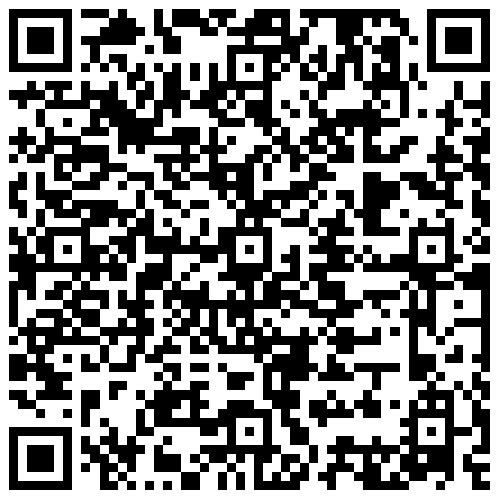
\includegraphics[scale=0.3]{eduroamqrcode}
%%https://www.unibo.it/it/servizi-e-opportunita/studio-e-non-solo/wi-fi/eduroam-education-roaming

\subsection{大学周边}
大学周边商店,即UniboStore,销售各式各样含有大学元素的商品。其出售的Alma Mater Studiorum服装和配饰系列是与从事体育运动的国内和国际领先公司Macron合作创建。
如果想要购买,可以选择网上浏览或者前往线下商店。\\
官网地址:https://www.unibostore.it/\\
商店地址:Piazza Verdi, 2/A - 40126 - Bologna\\
营业时间:周一至周五 9:00-19:00

\subsection{图书馆系统}
\subsubsection{SBA}
大学图书馆系统 - SBA,是负责协调图书馆、图书收藏以及书目和文献服务的大学机构,博洛尼亚大学几乎每个学院都有图书馆。如果你想要借阅图书,可以通过图书馆官网首页的检索系统查找是否有这本书、在哪个图书馆、并且可以在线预约领取时间。大学同样拥有数量即为可观的电子版资源和文献。\\
官方网站:https://sba.unibo.it/it\\
\subsubsection{SBN/UBO}
同时大学还和大区及市立图书馆合作,成立了SBA/UBO系统方便博洛尼亚大学的学生使用,其官网主页同样拥有检索系统。\\
官方网站:https://sol.unibo.it/SebinaOpac/.do

\subsubsection{AlmaRE}
AlmaRE拥有意大利境内最大的数据库、电子期刊和电子书集合,也涵盖了利基学科领域。其拥有:\\
超过5万种电子期刊;超过370个书目、全文、事实和引文的数据库;超过64万本电子书,包括手册、百科全书、词典、参考书等。\\
同时大学还和包括剑桥大学出版社、美国化学学会、《自然》杂志,中国知网等几十家权威学术机构合作并订购了资源。\\
要查看更多信息,请访问AlmaRE官网:\\
https://sba.unibo.it/it/almare\\
要查阅资源,请访问其检索系统:\\
https://almastart.unibo.it/primo-explore/search?vid=39UBO\_VU\\
\textbf{注意!}有关中国知网的资源,请检索“CNKI”。

\subsection{软件折扣}
\subsubsection{Prezi}
Prezi是一个允许您以简单直观的方式创建演示文稿的系统。每个带有.pez扩展名的演示文稿都可以从具有Internet连接的任何计算机投影,或者,如果脱机或保存在USB设备上,则可以通过程序为Windows和Mac环境自动生成的播放器投影。\\
对于博洛尼亚大学的学生,通过机构电子邮件name.surname@studio.unibo.it注册,可以免费获得EDU Enjoy版本,并以折扣价获得EDU Pro版本。\\
注册网址:https://prezi.com/pricing/edu/

\subsubsection{MATLAB}
MATLAB - 校园许可证:根据与MathWorks的协议,大学已激活MATLAB Campus许可证,所有教授、研究人员、技术管理人员、合同教授、博士生、研究员和学生都可以在自己的计算机上安装MATLAB和Simulink应用程序,并参加免费的在线培训课程。\\
MATLAB是一个用于数值计算、统计分析和仿真的开发环境,全球有数百万人使用,其主要用于经济学、工程、数学、物理、医学、生物学等领域。Simulink是用于多域仿真和基于模型的设计的图形环境,与MATLAB集成。\\
该软许可证可供博洛尼亚大学社区的所有成员使用,包括:教授、研究人员、技术管理人员和学生,简而言之拥有大学凭证(@unibo.it 或@studio.unibo.it)的成员。\\
该许可证包括MATLAB和Simulink应用程序以及工具箱。完整列表可在其官网的博洛尼亚大学页面上找到。该许可证包括来自 MathWorks 的技术支持(使用电子邮件地址support@mathworks.it)。也包括了提供免费的在线培训课程。\\
\textbf{注意!}仅允许用于教育或公共研究活动(结果必须是公开的,而不是公司专有的)。因此它不能用于商业活动。安装软件的机器必须归博洛尼亚大学或个人所有。不允许安装在其他机构或研究中心的计算机上,即使大学与他们有持续的合作。\\
注册网址:https://it.mathworks.com/academia/tah-portal/alma-mater-studiorum-universita-di-bologna-1122528.html

\subsubsection{Microsoft Office 365}
根据与微软的协议,博洛尼亚大学的所有学生都可以免费使用Office365套件。\\
Office 365是一套个人生产力工具,包括电子邮件管理、专业编辑、电子表格和演示文稿管理、文档共享等。\\
Office 365可供所有在博洛尼亚大学定期注册的学生使用,并可通过他们的大学凭证 (@studio.unibo.it) 在portal.office365.com上访问。当学生与大学的关系终止后,将保留仅使用电子邮件的可能性。\\
随着研究的结束,通过博洛尼亚大学与Microsoft的协议安装在个人计算机上的Office产品许可证的有效性也将终止。要继续使用产品,您必须根据微软的商业条件购买许可证。\\
大学提供的许可证包括:
\begin{itemize}
 \item 能够使用Office 的在线版本,其中包括例如Word、Excel、PowerPoint、Outlook(邮件、联系人、日历、任务);
 \item 能够下载和安装最新版本的Office; 
 \item 访问Onedrive:用于在所有设备上编辑和共享的文档、照片和视频的云存储空间;
 \item Skype for Business:即时通讯软件、音频和视频通话、在线会议和演示、可用性信息和共享,供您在组织内使用。
\end{itemize}
要下载并使用Office365套件,请访问微软官网,并使用你的大学凭证(即登录Studenti online的账户)登录。\\
微软官网:https://www.microsoft.com/

\subsubsection{STATA SE}
STATA SE - 校园许可证:根据与TStat的协议,大学已激活STATA SE Campus许可证,所有教授、研究人员、技术管理人员、合同教授、博士生、研究员和学生都可以在自己的计算机上安装STATA SE应用程序,并参加免费的在线培训课程。\\
Stata 是一款综合统计软件,其功能能够满足经济学、社会学、心理学、生物统计学、流行病学等学科的广泛学术和专业用户的需求。Stata包括广泛的统计功能和完整的数据管理功能。它对于新手用户来说很容易使用,但为更有经验的用户提供了复杂的编程选项。新开发的功能和官方更新只需通过互联网即可安装。\\
该软件可供博洛尼亚大学社区使用:教授、研究人员、助教人员、兼职教授、博士生、研究员和具有机构资格的定期注册学生,简而言之拥有大学凭证(@unibo.it 或@studio.unibo.it)的成员。\\

要在您的计算机上安装该软件,请参阅https://www.unibo.it/secure/software-stata/页面。该软件适用于各种操作系统。\\

\textbf{注意!}校园许可证包括STATA SE应用程序。该许可证是个人许可证,不得转让给第三方,并且允许最多三次安装,前提是这些安装是在供个人专用的机器上进行的(最常见的示例:办公室、家庭、笔记本电脑)并且不同时使用。该许可证包括TStat的技术支持(有关技术支持,联络tstat@tstat.it)。\\

此外,大学教授和员工可以选择通过Prof+Plan学术计划购买/升级永久或年度单用户SE或MP2许可证,与学术许可证的标准价格相比,成本降低约48\%。\\

安装该软件的计算机必须属于博洛尼亚大学或个人所有。即使大学与其他机构或研究中心正在进行合作,也不允许在其他机构或研究中心的计算机上安装。


\subsubsection{其他}
很多软件对学生都有折扣和优惠,例如ADOBE旗下的软件、Cinema 4D、AutoCAD等,有关信息请访问各软件官方网站查看。

\subsection{如果您是一位母亲}
博洛尼亚大学拥有向母亲开放的母乳喂养区,对女学生、教师、技术管理人员、博士生、研究员和任何需要安静空间来母乳喂养的新妈妈们、以及她们的探亲家庭成员(例如在毕业典礼期间)开放。\\
空间内有:更衣台、水槽、奶瓶加热器、一个供年长兄弟姐妹使用的小型游乐区和一个供陪伴他们的人使用的等候区。\\
地址和时间:\\
Via B. Andretta, 4 (ex-Belmeloro 10-12) Bologna\\
开放时间:周一至周五 9:00 至 19:00\\
Via Zamboni 33 Bologna, 即il Museo di Palazzo Poggi\\
开放时间:周二至周五 10:00 至 16:00 - 周六和周日 10:00 至 18:00\\
Via Zamboni, 63 Bologna, 即la Collezione di Geologia “Museo Giovanni Capellini”\\
开放时间:周二至周五 10:00 至 16:00 - 周六和周日 10:00 至 18:00\\








